\documentclass[11pt, a4paper,twocolumn]{article}
\linespread{1.3} % 1.5 spacing
\usepackage{amsmath}
\usepackage[margin=0.5in]{geometry}
\usepackage{graphicx}

\title{\textbf{Control Systems - ELEN90055} \\ \textit{Workshop 4}}
\date{2018\\ Semester 1}
\author{George Juliff -- 624946\\Kweku Acquah -- 741573\\Thomas Miles -- 626263}




\begin{document}

\maketitle
\pagenumbering{gobble}
\clearpage
\pagenumbering{arabic}
\section{Introduction}\label{sec:intro}
This project aims to create a feedback controller in order to balance an activated inverted pendulum in an upright position whilst rejecting various disturbances.

To achieve this goal, Simulink was used to interface with the robot the pendulum was mounted on, adjusting the controller configuration and parameters, sending commands, and receiving encoder data from the robot's motors as well as data from a gyroscope mounted on the pendulum. This allowed a wide range of variables to be tested to systematically assess their impact on the system behaviour, aiding in design decisions when choosing the final controller configuration.

%-----------------------------------------------------------------------------------------------------------------------------%
\section{System Modelling}\label{sec:model}
	
%	Kweku's section goes here.



%-----------------------------------------------------------------------------------------------------------------------------%
\section{	Controller Design	}\label{sec:design}

	\subsection{	Performance Requirements	}
	% 
	
	\subsection{	Controller Implementation	}

	% Controller equasion used
	% Brief overview of the type implemented and why it was chosen

	\paragraph{		Plant Model Considerations		}
			% Impact of adding poles and zeros using root locus
			% Note the closed loop controller using only proportional gain
						
			
	\paragraph{		Loop Shaping		}
			% Bode plot of plant, note what the controller needs to do to meet phase and gain spec
			% As such, explain how the choice of pole/zero placement generated desired results using bode/rlocus/nyquist
			% Validate internal stability			
			
	\paragraph{		Time Domain Response		}
			% Show the system behaves as desired based on impulse and step responses.
			
	
			
%-----------------------------------------------------------------------------------------------------------------------------%
    \section{Implementation and testing}\label{sec:test}
        \subsection{Presentation of performance}\label{subsec:performance}

	\begin{figure}[h!]
	\begin{center}
	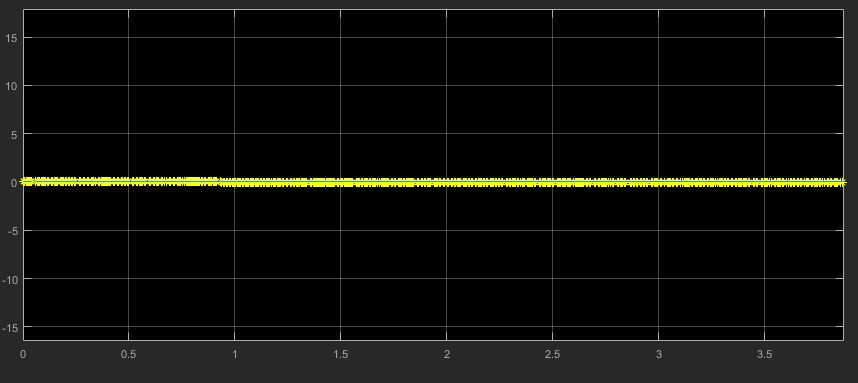
\includegraphics[width=\linewidth]{Undisturbed}
	\caption{Stable system without disturbance}
	\label{fig:4.1}
	\end{center}
	\end{figure}
From figure \ref{fig:4.1} it can be seen that under optimal conditions the system is perfectly stable. However, as it is possible to balance the arm in this position without the motor being driven this is not a difficult state to maintain. In figure \ref{fig:4.2} the state the arm returns to when removed from this base state is shown.
	\begin{figure}[h!]
	\begin{center}
	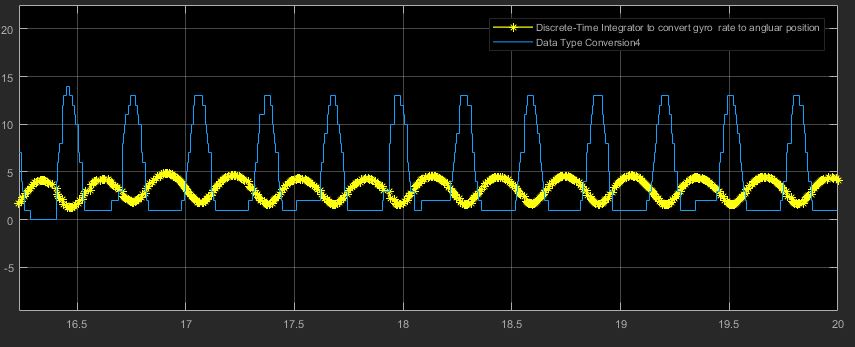
\includegraphics[width=\linewidth]{Ocilation}
	\caption{Return state after disturbance}
	\label{fig:4.2}
	\end{center}
	\end{figure}
While the oscillation was not expected the arm is able to maintain this state indefinitely and can therefore be considered to have remained upright.

        \subsection{Assessment of design criteria}\label{subsec:assessment}
            \subsubsection{Regulation and Disturbance Rejection}
	\begin{figure}[h!]
	\begin{center}
	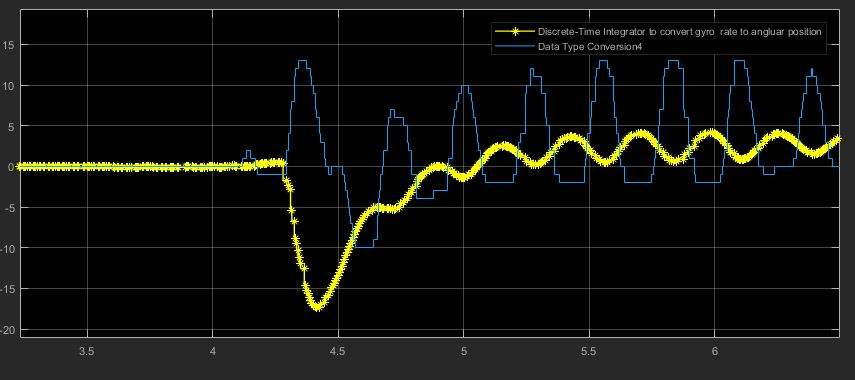
\includegraphics[width=\linewidth]{ImpulseDisturbance}
	\caption{Impulse response}
	\label{fig:4.3}
	\end{center}
	\end{figure}
Figure \ref{fig:4.3} demonstrates the systems ability to recover from an impulse disturbance. As previously mentioned it does not recover from the oscillation, although it is able to maintain the upright position this criterion was considered fulfilled.

	\begin{figure}[h!]
	\begin{center}
	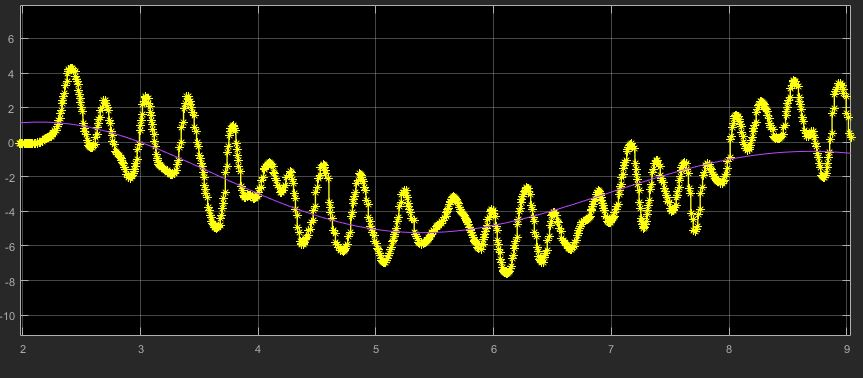
\includegraphics[width=\linewidth]{Steering}
	\caption{Steering resposnce}
	\label{fig:4.4}
	\end{center}
	\end{figure}
For the case of the system in steering mode in figure \ref{fig:4.4} the result is not so clear. While the high frequency oscillation did not present a problem there also a much lower frequency oscillation that, when compared with the steering angle in figure \ref{fig:4.5}, can be seen to be related.

	\begin{figure}[h!]
	\begin{center}
	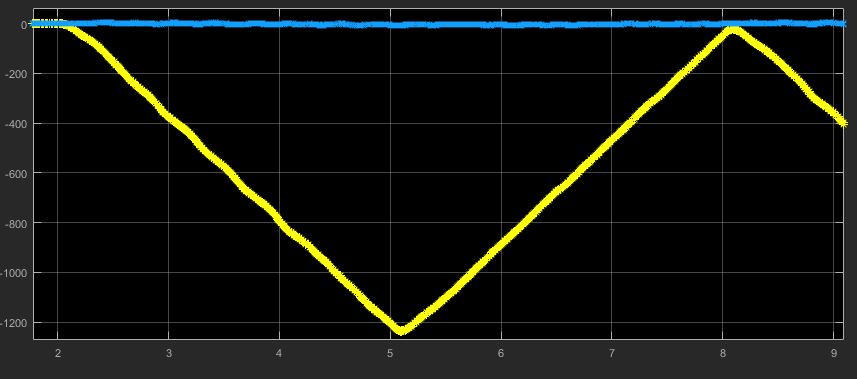
\includegraphics[width=\linewidth]{SteeringWheels}
	\caption{Steering wheel angle}
	\label{fig:4.5}
	\end{center}
	\end{figure}
While it may appear that were the turning to continue the system may fail, it can be seen this is not the case in figure \ref{fig:4.6}. Ignoring the high frequency noise, a lower frequency oscillation can be seen opposing the movement of the arm. From this it can be inferred that were the steering to continue then the system would remain an equilibrium where the centripetal force is balanced by the motor.
	\begin{figure}[h!]
	\begin{center}
	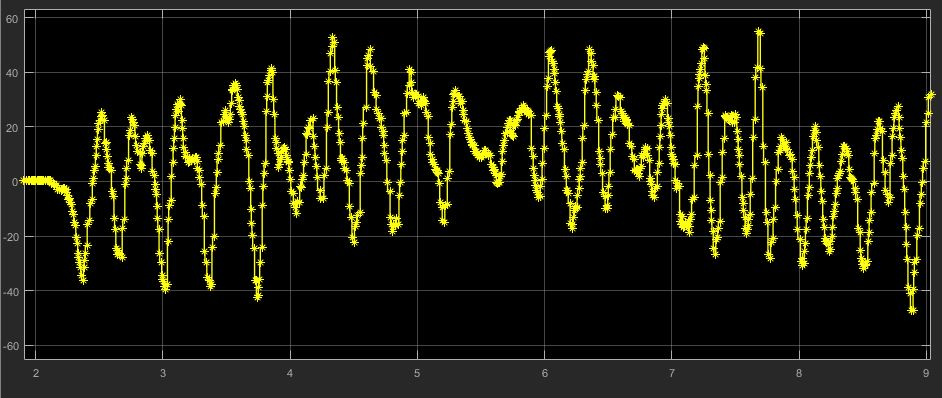
\includegraphics[width=\linewidth]{SteeringVoltage}
	\caption{Motor Driving Voltage}
	\label{fig:4.6}
	\end{center}
	\end{figure}

            \subsubsection{Phase Margin}
Unfortunately, the phase margin could not be shown to be 40$^\circ$. Adding a delay in the system corresponding to 40$^\circ$ at the critical frequency was the method used to test this, however, this resulted in the motor voltage repeatedly saturating and very erratic behaviour. This was due to the fact the maximum force that could be delivered by the motor was not taken into account during the design stage, and as such some boundary cases that may have appeared stable are not reliably so in practice.
	\subsubsection{Bandwidth}
The bandwidth requirement could also not be shown to be fulfilled, however, this was due to an inability to test it rather than because it necessarily wasn’t. The method of testing this would have been to introduce an 50rad/s signal and observe that its magnitude was reduced by more than $\sqrt{2}$. The issue was that the background oscillation of the system either overwhelmed the response for low disturbance magnitudes, or that the motors force limitation would cause the entire system to fail at high magnitudes. As such this criterium could not be verified one way or the other.

        \subsection{Comparison against simulated system}\label{subsec:comp}

	\begin{figure}[h!]
	\begin{center}
	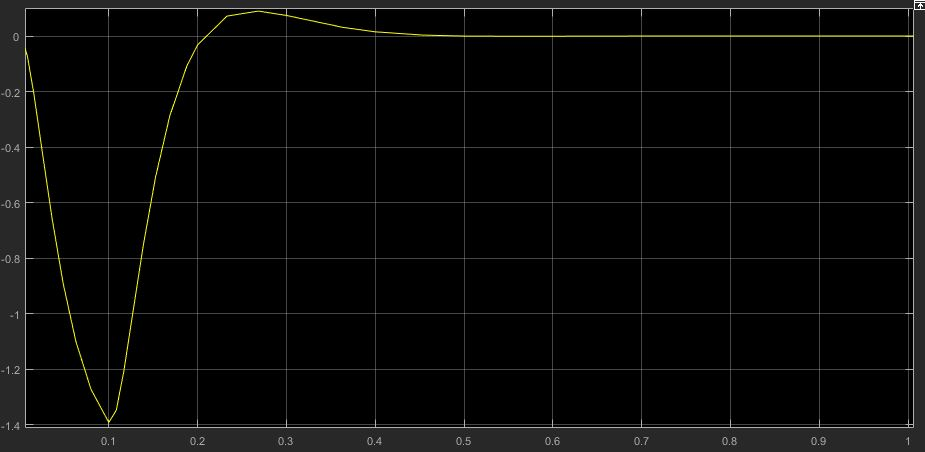
\includegraphics[width=\linewidth]{ImpulseSim}
	\caption{Simulated impulse response}
	\label{fig:4.7}
	\end{center}
	\end{figure}
Figure \ref{fig:4.7} shows the predicted impulse response of the system, and when compared to figure \ref{fig:4.3} several differences can be observed. Most immediately the oscillation present in the system is absent from the model. In addition, it is clear the system is significantly more damped than the model as on returning to steady state the system displays no overshoot and is significantly slower to do so.

There are several reasons this might be the case. The damping effect is likely primarily due to the unmodeled limitations of the motor rather than any real damping. The motor is unable to apply the full expected force that is applied in the model and this results in a damping like effect when the controller voltage saturates.

The oscillation on the other hand is likely caused by the assumptions made during the modelling. Namely the assumption that the motor is completely fixed. In reality it could be seen that the motor was able to shift in the robot, and in addition the entire robot would shift with the pendulum. This added motion was not accounted for and likely the primary reason for the oscillation although there were doubtless other contributing factors.

    \section{Conclusion}\label{sec:con}

While we were unable to demonstrate that all of the criteria discussed in \ref{sec:design} were met, we were able to demonstrate through experiment and calculation that the system is robust and stable. Furthermore we analysed and discussed the shortcomings of our control system, and why the realised system behaves differently to the modelled one.

Improvements could certainly be made to the model in order to better fulfil the design criteria. However better modelling the system would exponentially increase the mathematical complexity of the problem, and as such further experimentation my be the best way to find an improved model.


\end{document}
